\documentclass{styles/svproc}
\usepackage{url}
\usepackage{makeidx}
\usepackage[utf8]{inputenc}
\usepackage{graphicx}
\graphicspath{ {img/} }

\begin{document}

\title{Fine 3D path following of a quadcopter}
\author{Manuel Zafra Villar\inst{1} \and Jose María Cañas Plaza\inst{2}}
\institute{Universidad Rey Juan Carlos, Madrid, Spain}
\titlerunning{Fine 3D path following of a quadcopter}
\maketitle

\begin{abstract}
This paper addresses the design and implementation of a path following controlling system for a drone which relies on 3D localization by visual markers. The program is designed only for indoor flight, special attention is paid to accuracy of the position estimation algorithm, robustness of the path following controller and real time operation. The system is composed of two components, one responsible of the image analysis and 3D pose estimation and another responsible of the drone navigation. The system has been experimentally validated both in Gazebo simulator and in a real drone. 
\end{abstract}

\section{Introduction}

	In recent years, the rapid development of new technologies and the decreasing price of the hardware have allowed people an easier access to robotics. There has also been an emerging interest in the use of \textit{Unmaned Aerial Vehicles} (UAVs) on applications such as 3D mapping, military tasks, security, inspection \cite{nikolic2014} or agriculture. Maybe quadrotors are the most popularized aerial vehicles now. Currently there are several lines of research and projects with UAVs, like \textit{Project Wing} from \textit{Google} or \textit{Prime Air} from \textit{Amazon}. 

	In order to accomplish some of the above mentioned taks, the vehicle must work autonomously without the constant supervision of human operators. One approach to achieve this autonomy the UAV is following of predefined paths in 3D \cite{dandrea2015,beul2015}. For this the UAV should continuously know its 3D position. Outdoor this can be achieved with the help of sensors such as GPS, Inertial Measurement Unit (IMU) or altimeter. For indoor environments higher accuracy is needed as there may be multiple obstacles within a few meters. 
	
	Solutions to 3D localization may come from external motion capture systems \cite{jimenez2014,lupashin2014} of from onboard computer vision \cite{wu2013}. Typically motion capture systems monitor the position of the vehicles at a frequency of 100 Hz. The procedures may vary depending on the camera used (RGB, RGBD, ToF...) and whether the camera is on the scenario or onboard the drone. Three main techniques can be distinguished for onboard cameras. First, \textit{Visual Odometry} in which the position is estimated by calculating the incremental movement between separate pictures extracting the characteristic points of an image. Even though this method can provide good short-term accuracy, the error rapidly increases with movement. Second, \textit{Visual SLAM} family of algorithms allows the mapping of the area observed and simultaneously the localization of the camera. MonoSLAM, PTAM, DSO \cite{engel2017}, LSD-SLAM and SVO \cite{forster2014} algorithms belong to this family. And third, \textit{Localization based on Markers}, fiducial systems, which are based on the previous knwoledge of the environment's map \cite{apvrille2013,lopezceron2016}. This information is given by a series of visual markers so when the camera detects any of these markers the relative position to it can be obtanied, therefore the global position of the camera. 
%The markers that can be used are plenty, with the only limitation being that the camera must be able to recognize them easily. Some of the most common markers used are bi-dimensional bar codes, which are the ones used by this system.
	


        %% hardware: drones 
        %% In this case, we are using a specific UAV type, quadcopters. A quadcopter is a multirotor helicopter that is propelled by four rotors. This kind of aerial vehicle differs from conventional helicopters, which use rotors that are able to vary the pitch of their blades dynamically as they move around the rotor hub. Usually, the architecture consist of two rotors on the front and two on the back, however some models include one frontal rotor, two on the sides and another one on the back. The rotors, when functioning, apply an upwards force called lift that sustain the vehicle. In order to the quadcopter to take off, the lift must be higher than gravitational forces. Once hovering, if gravitational forces equal lift, the vehicle will remaing still. Modifying lift will cause it to go upwards or downwards depending on the force applied. Horizontal movement is generated by altering the rotation power of two pairs of rotors. For instance, if we want to apply forward movement we have to reduce the power of the two frontal rotors and increase power on both of the rear rotors. The difference of the power applied is proportional to the movement speed generated. To understand rotation movement, we have to comprehend how the rotors work in sense of rotational direction. In order to the quadcopter to mantain its position, angular velocity must equal zero. This is accomplished by having two rotors function with one rotational direction and making the opposite pair rotate on the reverse direction. If different power is applied to pairs of rotors, the quadrotor will rotate towards the direction of the most powerful rotors.
	
	The goal of this project is to develop a vision-based autonomous navigation system for a quadcopter in indoor environments. The navigation will be based on a path tracking method, ensuring a robust position control. In order to accomplish that, self location will depend on computer vision algorithms relying on visual markers. Given the characteristics of the environment, the system must function with minimal error in order to avoid obstacles in close spaces.

\section{Infrastructure}

Several hardware and software pieces have been used in this work.

\subsection{ArDrone2 quadrotor}

	The platform used is \textit{Parrot}'s \textit{ArDrone2.0}. The quadcopter was developed in 2012 as an enhanced product of its precessor, \textit{ArDrone1.0}. The onboard computer runs a \textit{Linux} OS, and communicates with the pilot through a self-generated Wi-Fi spot. The onboard sensors include an ultrasonic altimeter enhanced with an air pressure sensor, as well as 3-axis gyroscope, accelerometer and magnetometer, which are used to provide stabilisation. It is also equipped with a 720p front camera and a ventral QVGA sensor.
	
	\begin{table}
	\centering
	\setlength\tabcolsep{7pt}
	\caption{ArDrone2.0 Characteristics}
	\begin{tabular}{llllll}
	\hline\noalign{\smallskip}
	Characteristic  & Value\\
	\noalign{\smallskip}
	\hline
	\noalign{\smallskip}
		Size & 58.4 x 1.3 x 58.4 cm. \\
		Weight & 436 g. \\
		Wi-fi range & 50 m. \\
		Max. speed & 18 km/h \\
		Camera  & 1280 x 720 pixels \\
		Max. height & 100 m.\\
	\hline
	\end{tabular}
	\end{table}

\subsection{AprilTags beacons}

	\textit{AprilTags} is a visual fiducial system widely used for tasks including robotics, augmented reality and camera calibration. This system was developed in 2011 by Ed Olson \cite{eolson}. The concept is similar to QR Codes in that they are two-dimensional bar codes (Fig. \ref{fig:apriltags}). However, AprilTags are designted to encode far smaller data payloads (between 4 and 12 bits) and it introduces a new encoding system addressing some specific problems with 2D bar codes, enhancing robustness for rotation angles detection and against false positives, and allowing them to be detected from longer ranges.
	
	The AprilTags detection software detects any AprilTags in a given image, providing the unique ID of the tag as well as its location in the image. It can also provide the the relative transformation between tag and camera. For this system, AprilTags has only been used for the detection of tags in an image, obtaining the tag ID and the location (height and width pixel) in the given image. The positon estimation given by this library is not used because we wanted to obtain the postion given solely by our own developed component.
	
	\begin{figure}[h]
		\begin{center}
		{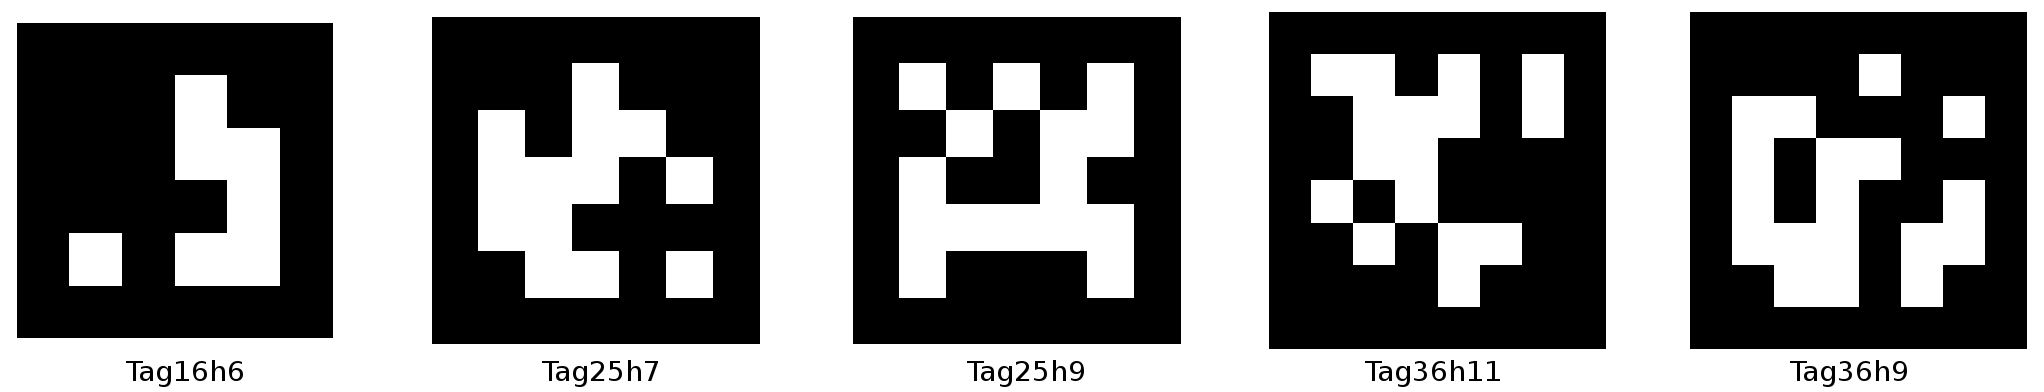
\includegraphics[width=\linewidth]{ejemplosapriltags.png}}
		\end{center}
		\caption{Some examples of AprilTags markers}
		\label{fig:apriltags}
	\end{figure}
	
\subsection{JdeRobot framework}

	The system has been developed using the JdeRobot software framework, a robotics and computer vision development platform. It provides support to many sensors and actuators, while providing several libraries and drivers. It is mainly developed in C++, also having some parts developed in Python. In JdeRobot a robotic application typically is composed of several interacting components and the communication between them is done through \textit{Internet Comunication Engine} (ICE) over TCP/IP. ICE is a server-client protocol, based on \textit{Remote Procedure Call} (RPC), which allows remote execution of software without worrying about communications.

 The components may extract information from different robot sensors and provide it for other components. Within JdeRobot there are many drivers developed to support several physical sensors and adapters. This simplifies hardware access from applications providing an abstraction layer over the manufacturer's software such as \textit{Ar.Drone SDK} in \textit{ArDrone}. 

        \subsubsection{Progeo Library}
        
        JdeRobot also contains several libraries such as \textit{progeo}, \textit{jderobotutil} or \textit{geometry}. Progeo is a projective geometry library that offers functions that relate 2D and 3D points. Having the camera extrinsic and intrinsic parameters, obtained by calibration, we can obtain the projected 3D point of a 2D image point. With the \textit{project} function, we can project a 3D point in space into a 2D image. With the \textit{backproject} function the exact 3D point corresponding to a pixel can not be determined, but provides a ray in 3D space that contains the 3D point that projects on that pixel.

\subsubsection{CameraCalibrator}

	CameraCalibrator is a JdeRobot tool which obtains the intrinsic parameters of a camera. CameraCalibrator recieves camera images by ICE interface, and offers a simple user interface which simplify the calibration process. In its configuration file, settings can be modified such as calibration pattern, number of images taken or delay between images. The component uses OpenCV and its camera calibration methods and writes the output in a \textit{.yml} text file. This tools was used to obtain the camera parameters for the real ArDrone camera and the simulated camera.

	\begin{figure}[h]
		\begin{center}
                  {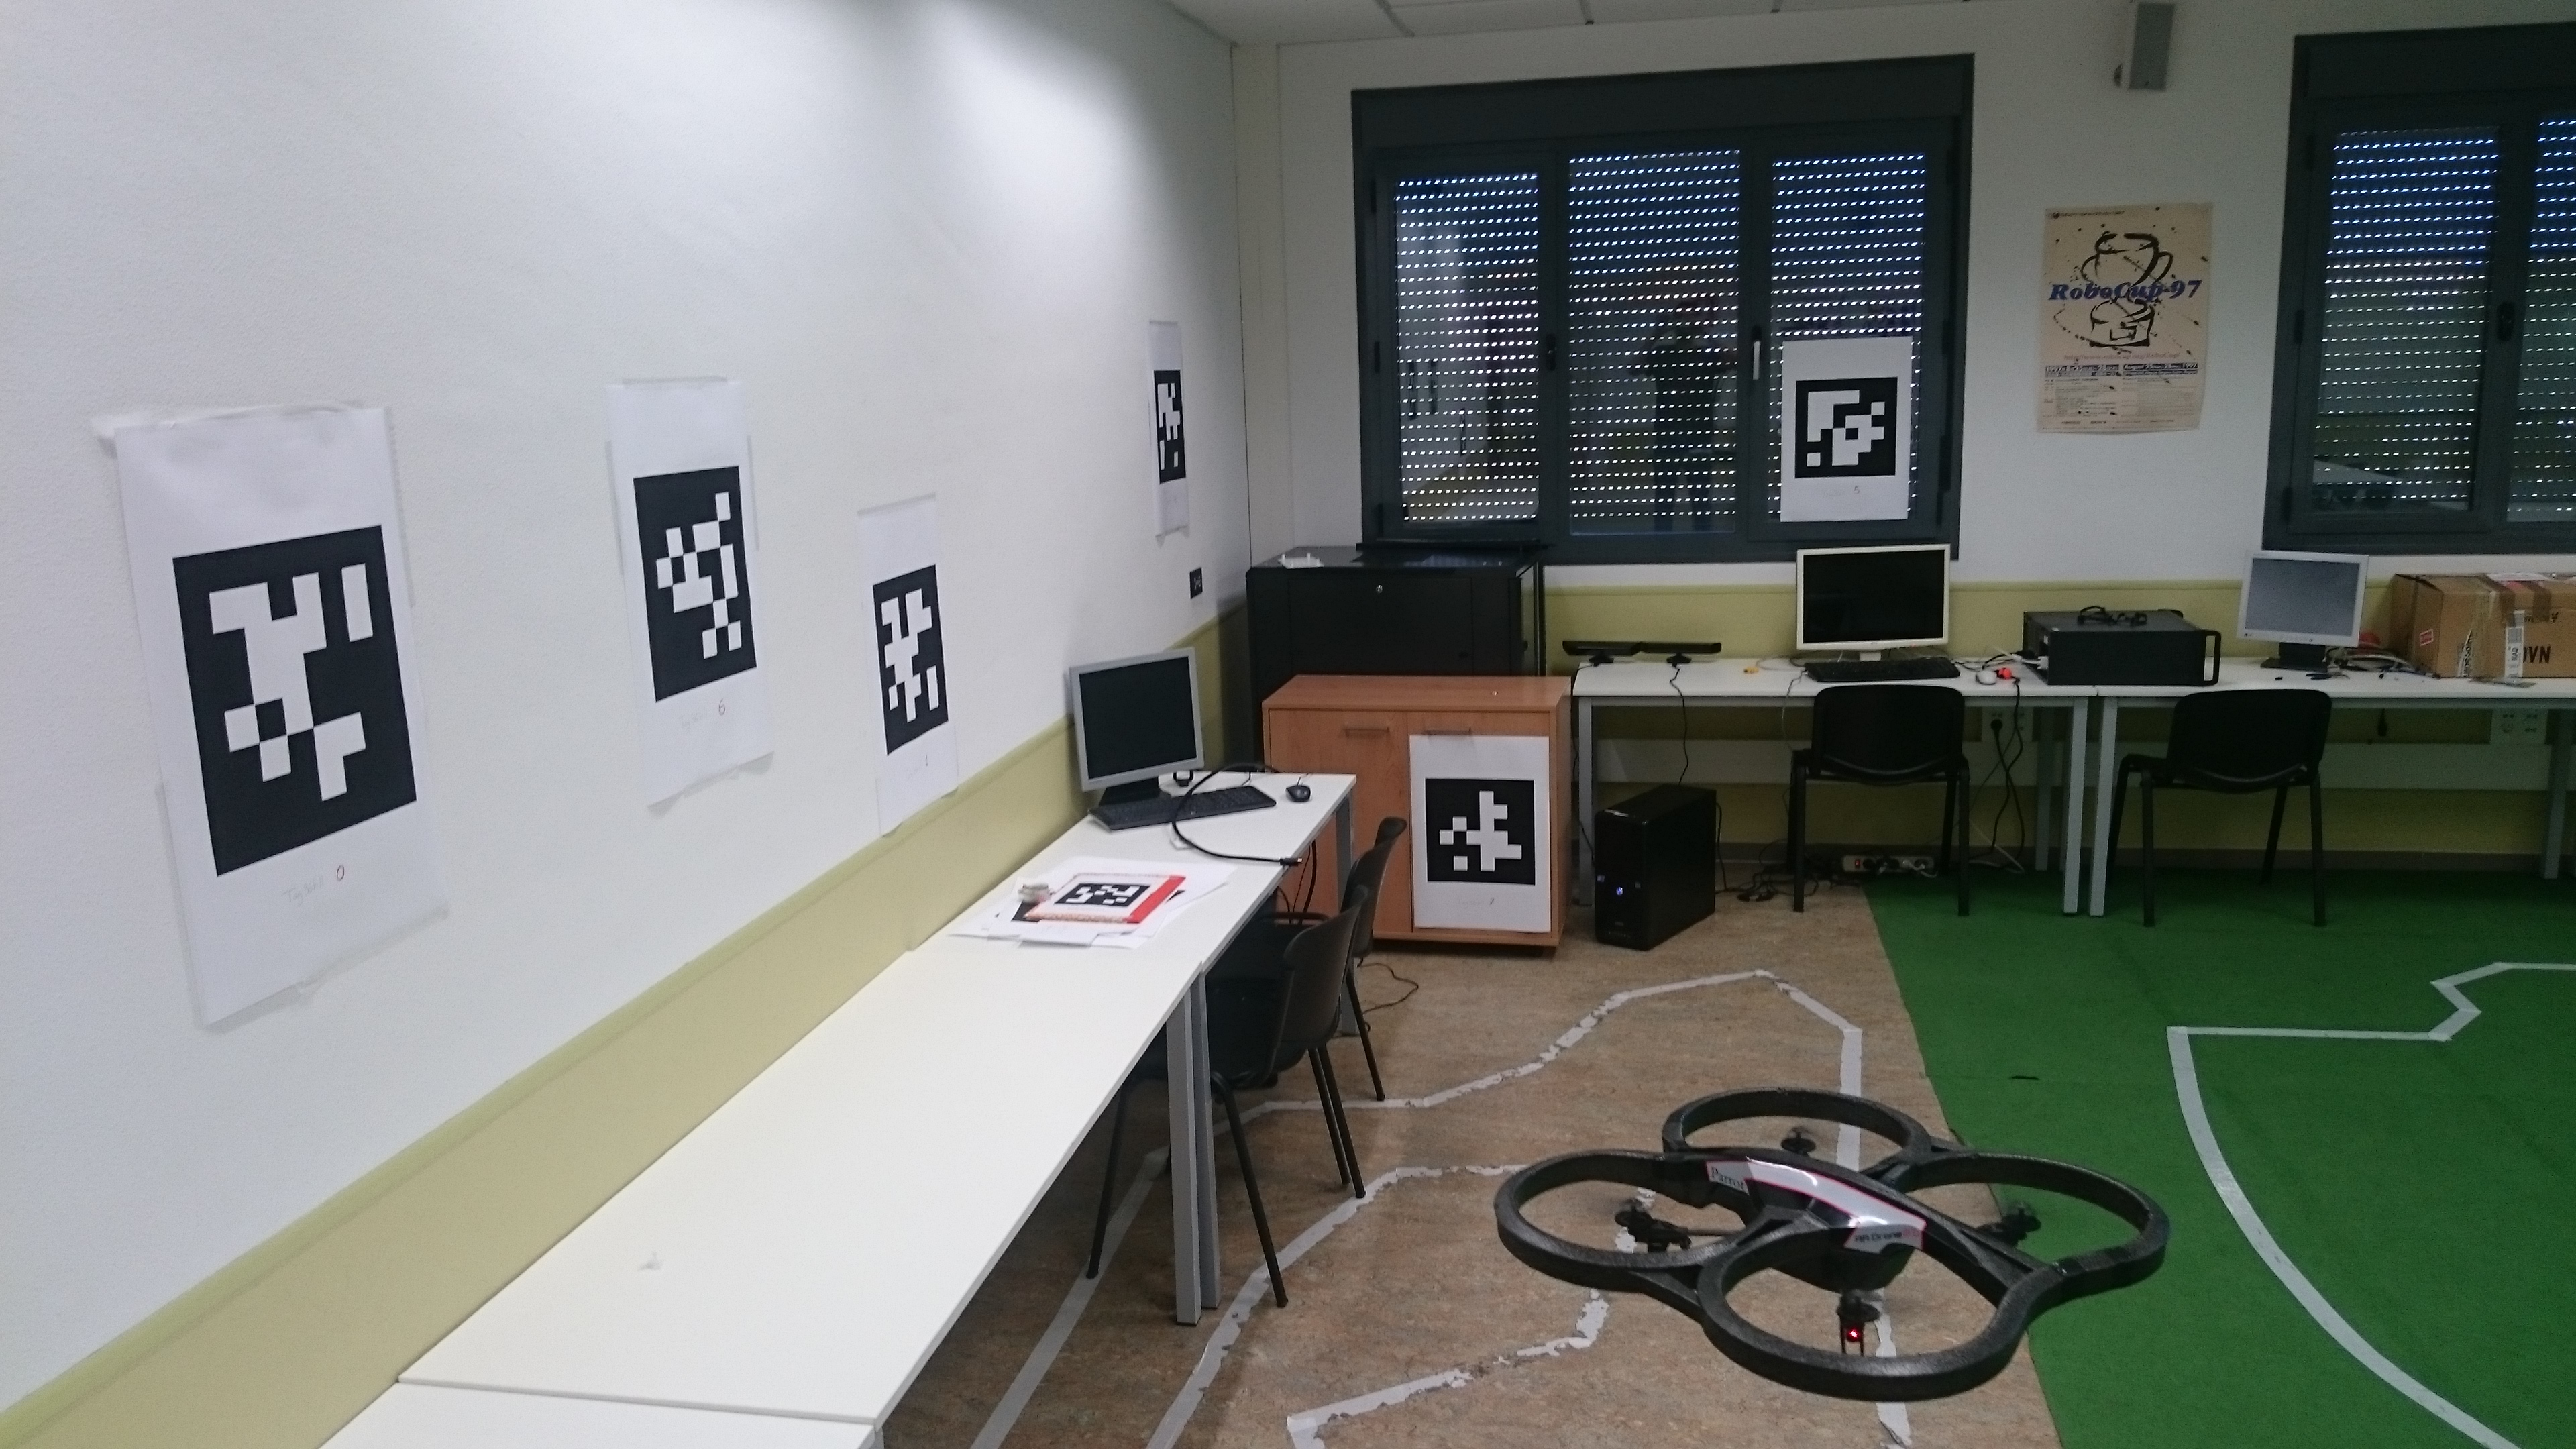
\includegraphics[width=6cm]{realnavigation.png}}
                  {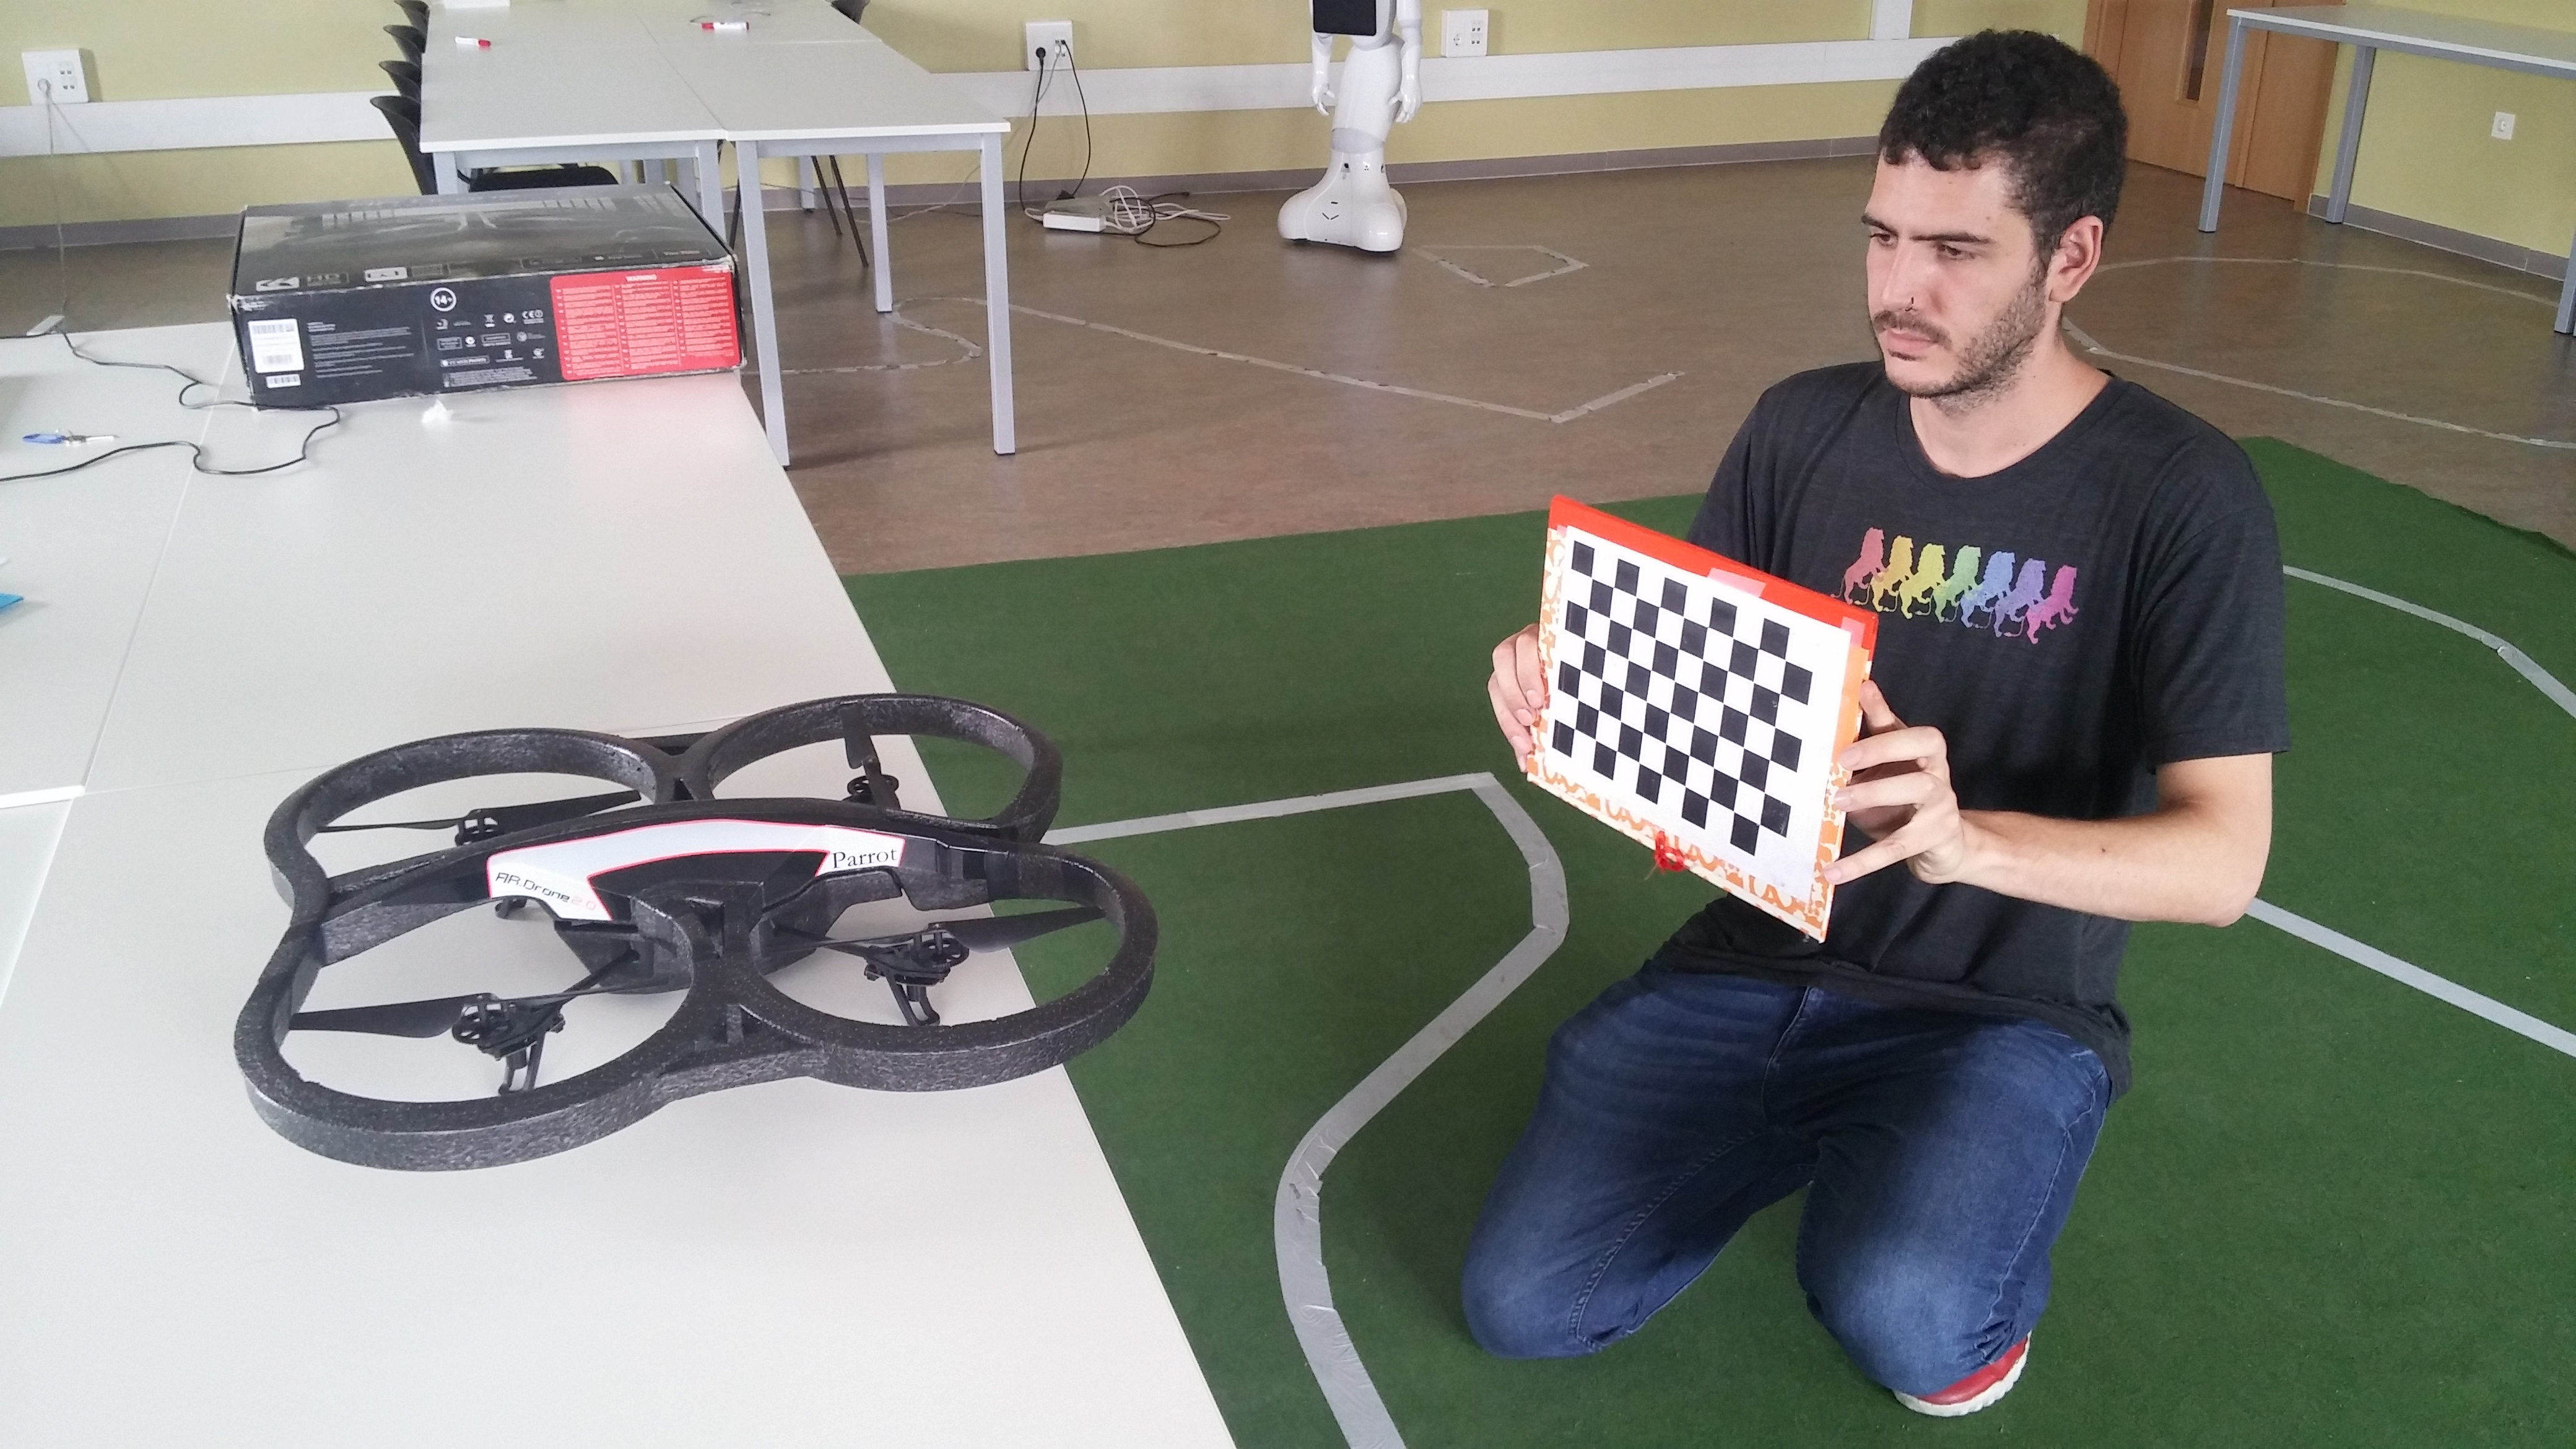
\includegraphics[width=6cm]{calibration.jpg}}
		\end{center}
		\caption{Real drone ArDrone2 and calibration of its onboard camera}
	\end{figure}

\subsubsection{Ardrone\_server}

	Ardrone\_server is one of the drivers included in JdeRobot that allows cammunication with the ArDrone device using ICE interfaces. The driver encloses the ArDrone SDK libraries provided by the manufacturer. There are six interfaces offered by the driver, three of them are designated for the information obtained by the sensors, two correspond to the actuators and the last one is for real-time configuration of the drone. The most important interfaces for this matter are \textit{CMDVel}, used to send velocity commands; \textit{Ardrone\_extra}, that allows execution of complex maneuvers methods like taking off or landing; and \textit{Camera}, where images captured by the camera are received.

\subsubsection{Uav\_viewer}

	Uav\_viewer is an application that allows the user the control of an ArDrone. It has a graphic user interface in which the information received by the quadcopter's sensors is displayed. It also has two control pads for the control of the drone's movement including vertical and horizontal speed as well as angular speed along the Z axis. The application can be use either with a real ArDrone as with a simulated quadrotor on Gazebo simulator.

\subsubsection{Quadrotor Gazebo plugin}

	Gazebo is a multi-robot simulator for both outdoor and indoor environments. It is able to simulate serveral robots with their sensors in a 3D world. This world can be created an personalized by the user, thanks to the tools provided for the integration with 3D models designed with SDF and the models included in Gazebo (\textit{TurtleBot} or \textit{Pioneer2}, from others). It is also able to simulate physical interactions between the objects in the 3D world thanks to its integration with physics libraries, such as \textit{Bullet} or \textit{Ogre}. The simulator is under constant development, under the \textit{Open Source Robotics Foundation}. Gazebo provides us with an extensive API, which is very well documented, to allow de users to develop their own plugins for their personalized robots and sensors. The simulator has been used to simulate the behaviour of the drone on the first iterations of the development stages. JdeRobot includes one plugin for a quadrotor similar to ArDrone2 from Parrot (Fig. \ref{fig:simnavigation}).


\section{3D path tracking system}

\subsection{System design}

The developed application is composed of two components, one of them is tasked with image analysis and position estimation and the other one manages drone's movement and control its position given the estimated location. Communication between components is done through ICE, same with communication between the application and the cuadricopter.
%Each component has several modules running with threads that have different time cycles. One module of each component is serving as communications interface and manages shared memory, and the other ones correspond to graphic interface, information processing, algorithm application, etc.
	
	First, \textit{VisualLoc} component receives the image taken by the quadrotor's camera. This component performs an analysis of the image looking for the presence of \textit{AprilTag} markers. Once the markers are located, if any, the component applies projective geometry algorithms in order to estimate the relative position of the camera to each of the markers found. Next operation is the application of spatial fusion by a weighted average filter that depends on the distance between the markers and the camera, giving higher weight to those closer to the camera. Finally, a temporal fusion is carried out by a \textit{Kalman Filter} and the estimation is sent to clients.

        Second, \textit{Navigator} component recieves the positions and generates a combination of velocities that control the movement of the quadcopter. The position control is based on a predefined path that the drone must follow. Given the horizontal characteristics of the indoor environments, the algorithm rests heavily on the rotation angle along the Z axis. The algorithm predicts the future position of the vehicle and adjust the steering angle so the future position error in relation to the path is minimized.

        \begin{figure}[h]
          \begin{center}
            {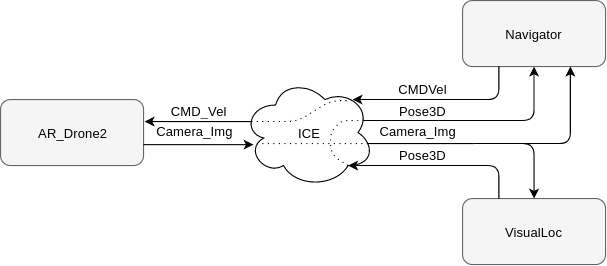
\includegraphics[width=\linewidth]{interactuacionproj.png}}
          \end{center}
          \caption{Global system design}
	\end{figure}
        
\subsection{Beacon based visual 3D localization}

	The self-location task is carried out by the component \textit{VisualLoc}. The software architecture of this component consists of a main module \textit{MainWindow} that interconnects the rest of the modules and implements an user graphic interface. One of those modules is \textit{Sensors}, which manages ICE interfaces and shared memory between the rest of the modules. MainWindow also contains instances of the \textit{CameraManager} and \textit{World} classes. \textit{CameraManager} is in charge for the computer vision algorithms and \textit{World} implements a 3D rendered world showing position estimation results. Following JdeRobot's standards, each of those modules are running on different threads that call the corresponding \texttt{update()} method. Calling this method causes the modules to carry out their main tasks in an iteration.
	
	A \textit{GeometryUtils} class has been developed in order to define a series of geometric calculus methods. Those methods include operations such as calculation of the intersection between planes and lines, generation of rotation matrices, or conversions between quaternions and euler angles. The structure that defines the camera is \textit{TPinHoleCamera} model, defined in \textit{JdeRobot}'s \textit{progeo} library. This structurel is based on a modelling where the projection is conical, meaning that all the light rays, at some point, go past one unique point, the camera focus. Pin Hole model is very useful thanks to its simplicity and precision in camera modelling. In order to instance a \textit{TPinHoleCamera} object, camera parameters must be obtained by previous calibration of the real camera. Information regarding markers position and camera parameters are loaded from text files, \textit{markers.txt} and \textit{camera.yml} correspondingly.
	
	% \begin{figure}[h]
	% 	\begin{center}
	% 	{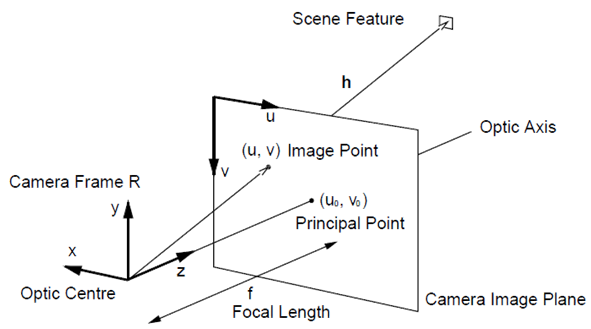
\includegraphics[width=\linewidth]{pinhole.png}}
	% 	\end{center}
	% 	\caption{Pin Hole Camera model}
	% \end{figure}
	
	
	The method \textit{ProcessImage} contained in \textit{CameraManager} has the task to process the 2D image captured by the camera looking for markers, as well as estimating the 3D position of the camera. The markers found are instanced by \textit{MarkerInfo} class, which contains the information about each marker: id, size and position. Position is stored in two matrices, one with the position of the marker regarding the world and another one with the position of the world regarding the marker. The \textit{AprilTags} detection method is applied to a greyscale converted image, this method generates an array containing all markers detected. The detected markers are highlighted on the original image and shown on the user interface.
	
	Once the detection array is created, each one of the markers are located on the original image and a series of geometric operations are applied. Those operations start with the application of \textit{OpenCV}'s function \textit{SolvePnP}, which returns the relative position of the camera given a reference system composed of the correspondence between the 2D image points and the referred world's 3D points. Thus the translation and rotation vectors that determine the position of the marker in relation to the camera are obtained. In order to acquire the full RT matrix, \textit{OpenCV}'s function \textit{Rodrigues} is used. The matrix containing the position of the camera referred to the world is obtained by multiplying the calculated matrix and the matrix of the position of the marker in relation to the world.
	
	The position estimations for each marker are stored in an array, then, a \textit{spatial fusion} is applied by a weight filter. This filter asign a different weight to each estimation based on the distance to the marker, so closer markers get a higher weight. Weight values were asigned by experimental testing, analysing the distances where the system lost accuracy. The filter extracts the weighted average of the estimations in the array and obtains a ratio for each estimation (\ref{eq:ratio}). Then, the final estimation is calculated applying that ratio to its corresponding estimation and summing all the resulting values(\ref{eq:xyzfusion}). There is a special operation with rotation angles, as they cannot be summed as the linear coordinates are (\ref{eq:alphafusion}).
	
	\begin{equation}
	ratio_{i} = \frac{weight_{i}}{weight_{total}}
	\label{eq:ratio}
	\end{equation}
	
	\begin{equation}
	[x,y,z]_{fusion} = \sum_{i=1}^{n} ([x_{i},y_{i},z_{i}] \cdot ratio_{i})
	\label{eq:xyzfusion}
	\end{equation}
	
	\begin{equation}
	\alpha_{fusion} = \arctan \left( \frac{ \sum ( \sin \alpha_{i} \cdot ratio_{i} ) }{ \sum ( \cos \alpha_{i} \cdot ratio_{i} ) } \right)
	\label{eq:alphafusion}
	\end{equation}
	
	

        %% To accomplish that, a \textit{Kalman Filter} has been implemented. This filter was developed by Rudolf E. Kalman \cite{kalman:re} and its fuction is to estimate the state of a dynamic system using a series of measurements observerd over time, containing statistical noise. If it is a Gaussian noise, it works as an optimal estimator minimizing cuadratic error. \textit{Kalman Filter} estimate the state of a process $x$ in a given time $k$ (\ref{eq:xk}), provided the measure $z$ (\ref{eq:zk}). Where $w_{k}$ represents process noise and $v_{k}$ represents measure noise, asumming they are white gaussian noise and mutually independent.
	
	%% \begin{equation}
	%% x_{k} = A \cdot x_{k-1} + w_{k-1}
	%% \label{eq:xk}
	%% \end{equation}
	
	%% \begin{equation}
	%% z_{k} = H \cdot x_{k} + v_{k}
	%% \label{eq:zk}
	%% \end{equation}
	
	%% $A$ matrix relates the current state with the previous state, while $H$ matrix relates state and measure. Therefore, the algorithm estimates the current state of the process based on the previous state while getting feedback with noisy measures. The filter's equations can be divided in two groups, state prediction equations and measure update equations.
	
	%% The prediction equations (\ref{eq:xkk})(\ref{eq:Pk}) are shown below, where $\hat{x}_{k}^-$ is the state estimated a priori; $\hat{x}_{k-1}$ the state estimated a posterori; $P_{k}^-$ is the error covariance a priori; and $P_{k-1}$ the error covariance a posteriori.
	
	%% \begin{equation}
	%% \hat{x}_{k}^- = A \cdot \hat{x}_{k-1}
	%% \label{eq:xkk}
	%% \end{equation}
	
	%% \begin{equation}
	%% P_{k}^- = A \cdot P_{k-1} \cdot A^T + Q
	%% \label{eq:Pk}
	%% \end{equation}
	
	%% The measure update equations (\ref{eq:Kk})(\ref{eq:xkkk})(\ref{eq:Pkk}), that can be acknowledge as measure correction equations are shown below, where $(z_{k} - H \cdot \hat{x}_{k}^-)$ is the residue and $K_{k}$ is the Kalman gain that minimizes error a posterori.
	
	%% \begin{equation}
	%% K_{k} = \frac{P_{k}^- \cdot H^T}{H \cdot P_{k}^- \cdot H^T + R}
	%% \label{eq:Kk}
	%% \end{equation}

	%% \begin{equation}
	%% \hat{x}_{k} = \hat{x}_{k}^- + K_{k} \cdot (z_{k} - H \cdot \hat{x}_{k}^-)
	%% \label{eq:xkkk}
	%% \end{equation}

	%% \begin{equation}
	%% P_{k} = (I - K_{k} \cdot H) \cdot P_{k}^-
	%% \label{eq:Pkk}
	%% \end{equation}
	
        Apart from the spatial fusion, a \textit{temporal fusion} is applied using a Kalman filter. With this method smooth results are obtained, while spike errors are eliminated. The variation of a single pixel may result in a sudden change in the position estimation, that is when the \textit{Kalman Filter} mitigates the sudden varations that may occur. The values of the noise covariance matrices must be obtained with experimental testing in order to obtain desirable results. The final position estimation obtained through this filter is sent to \textit{Pilot} component. Additionally, the 3D world shows the particular estimation for each marker and the filtered estimation.
	
\subsection{3D position control}

	Position control is accomplished by the component \textit{Navigator}. It consists of three modules, \textit{Interfaces}, \textit{Gui} and \textit{Pilot}. System inputs are \textit{Camera\_Img}, ArDrone's camera images to be shown in the user interface; and \textit{Pose3D}, position estimation given by \textit{VisualLoc}. The outputs are \textit{CMDVel}, composed of a combination of linear and angular velocities; and \textit{ArDrone\_extra}, where additional commands such as taking off or toggling cameras are sent to the quadcopter. Additionally, in simulation, the absolute position given by the plugin can be added as an input so the position estimation error can be calculated. The three modules posses an \texttt{update()} method that is called periodically by their corresponding thread asynchronically. With this method, each of the modules run an iteration carrying out their main tasks.
	
	\textit{Interfaces} is the module where ICE interfaces are created and managed. The parameters needed, such as IP address and port, are included in a text file that is loaded by ICE. This module also manages shared memory between the rest of the modules, administrating critical sections with a mutex. The next module is \textit{Gui}, which implements a graphical user interface. \textit{PyQt} is the library used for the implementation, following the standards of JdeRobot. The interface shows the images captured by the quadcopter's camera, a real-time graph, in which figures the error between the vehicle's position and the path, and a 3D world rendered with \textit{OpenGL}. This world shows the quadcopter's position in relation to a coordinate axis and the path to follow, as well as the vehicle's trail. Additionally, a series of buttons are implemented allowing the user to manipulate the quadcopter with actions such as pausing or resuming movement, taking off, landing and toggling cameras.
	
	The module \textit{Pilot} is where all the position information is processed and the velocity commands are generated. Initially, a simple navigation system was developed which only relied on direction vectors from the vehicle to the corresponding path point. After some experimental testing, we reached to the conclusion that steering angle along Z axis (yaw) is a key factor for an accurate navigation, whereas lineal velocity can be constant while not making a big impact. Additionally, the only linear velocity that matters are vertical velocity along Z axis and velocity along quadcopter's X axis, being velocity along quadcopter's Y axis irrelevant. Thus, developing a control system around the steering angle was the most suitable option. The algorithm is based on position prediction, so that steering angle adapts to the predicted error minimizing it. Only horizontal components are considered in the error prediction given the vertical components are minimal and don't affect steering control.
	
	The algorithm starts calculating the direction vector between the current position and the desired postion, that is the corresponding path point (\ref{eq:vecv}). Then, unit vector is computed (\ref{eq:uv}). In order to obtain the magnitude of the vertical and horizontal velocities while keeping linear velocity constant, unit vector must be decomposed. Vertical veloctiy is computed directly from the Z component of the unit vector and the predefined constant linear velocity $v_{k}$ (\ref{eq:vz}). Horizontal velocity is obtained by calculating the modulus of the X and Y component of the unit vector (\ref{eq:vxy}).

	\begin{equation}
	\vec{V} = \vec{P_{ath}} - \vec{P_{ose}}
	\label{eq:vecv}
	\end{equation}
	
	\begin{equation}
	\vec{u}_{v} = \frac{\vec{V}}{|\vec{V}|}
	\label{eq:uv}
	\end{equation}
	
	\begin{equation}
	v_{x} = |\vec{u}_{vxy}| \cdot v_{k}
	\label{eq:vxy}
	\end{equation}
	
	\begin{equation}
	v_{z} = |\vec{u}_{vz}| \cdot v_{k}
	\label{eq:vz}
	\end{equation}
	
	Next step is obtaining the horizontal distance the vehicle will travel until the next algorithm iteration. That distance is calculated from the horizontal velocity previously obtained and the lapse of time between iterations (\ref{eq:dtau}). In order to compute the future position regarding the current steering angle must be calculated. Considering that the received position rotation angles are expressed in quaternions, a transformation to euler angles must be done (\ref{eq:euler}). Once those values are calculated, future position point is obtained (\ref{eq:xf})(\ref{eq:yf}).
	
	\begin{equation}
	d_{\tau} = v_{x} \cdot \Delta_{t}
	\label{eq:dtau}
	\end{equation}

	\begin{equation}
	\theta_{z} = \arctan^2 \left( \frac{2 \cdot (q_{0} \cdot q_{3} +q_{1} \cdot q_{2})}{1-2 \cdot (q_{2}^2 + q_{3}^2)}\right)
	\label{eq:euler}
	\end{equation}		
	
	\begin{equation}
	X_{f} = d_{\tau} \cdot \cos \theta_{z} + x_{pose}
	\label{eq:xf}
	\end{equation}
	
	\begin{equation}
	Y_{f} = d_{\tau} \cdot \sin \theta_{z} + y_{pose}
	\label{eq:yf}
	\end{equation}
	
	In order to acquire the desired steering angle another factor must be obtained. That is the future lateral error, computed from the difference between the predicted future position and the desired path point(\ref{eq:le}). Finally, the steering angle is composed of the steering angle needed, $\delta{e}$, plus a steering angle gain that depends on the predicted future error (\ref{eq:deltatheta}). The steering angle needed is obtained by calculating the yaw angle needed by the vehicle to face the navigation point. The factor $K_{g}$ is the gain rate of the steering adjustment and must be obtained experimentally. This adjustment ensures a minimization of the error by correcting vehicle's trajectory and smoothing its movement. The velocity commands sent to the quadricopter through the method \texttt{CMDVel()} are $v_{x}$, $v_{z}$ and $\delta_{\theta}$. 

	\begin{equation}
	L_{fe} = - \sin \theta_{z} \cdot ( X_{path} - X_{f} ) + \sin \theta_{z} \cdot ( Y_{path} - Y_{f} )
	\label{eq:le}
	\end{equation}

	\begin{equation}
	\delta_{\theta} = \sin \delta_{e} +  K_{g} \cdot ( L_{fe} / v_{x} )
	\label{eq:deltatheta}
	\end{equation}

\section{Experiments}

% experimentos con drone simulado
	Experimental tests have been performed on simulated and real environments. The first tests were performed in \textit{Gazebo} simulator, creating a custom 3D world representing a flat where several AprilTags markers were placed. First experiments were conducted to both of the components inependently. Then, once validated, the full working system was tested first on simulated environments and then on a real scenario.
	
	Early self-localization experiments showed high levels of noise. Through analysis, the conclusion was that the algorithm was working properly but the parameters given to it were not. \textit{Kalman Filter} noise covariance matrices needed to be adjusted so the noise were modelled accordingly. Another problem was a faulty calibration of the camera used, which was easily solved by a more accurate camera calibration. Finally, one of the most important conclusions was that the markers needed to be bigger due to the difficulty in the markers detection process caused by the high mobility of the vehicle. The final marker size chosen was 25cm.
	
	On the control side, experiments showed good results. We had to run several iterations in order to find the proper parameters of the control algorithm. Vehicle's optimal speed is 0.1-0.4 m/s, and steering angle gain rate, $ K_{g}$ showed stable results within the range [0.1, 0.3]. The gain rate must be proportional to vehicle's speed in order to have a stable postion control. Lower gain rates are not enough to minimize the position error, while higher rates cause an erratic movement.
	
	\begin{figure}[h]
		\begin{center}
                {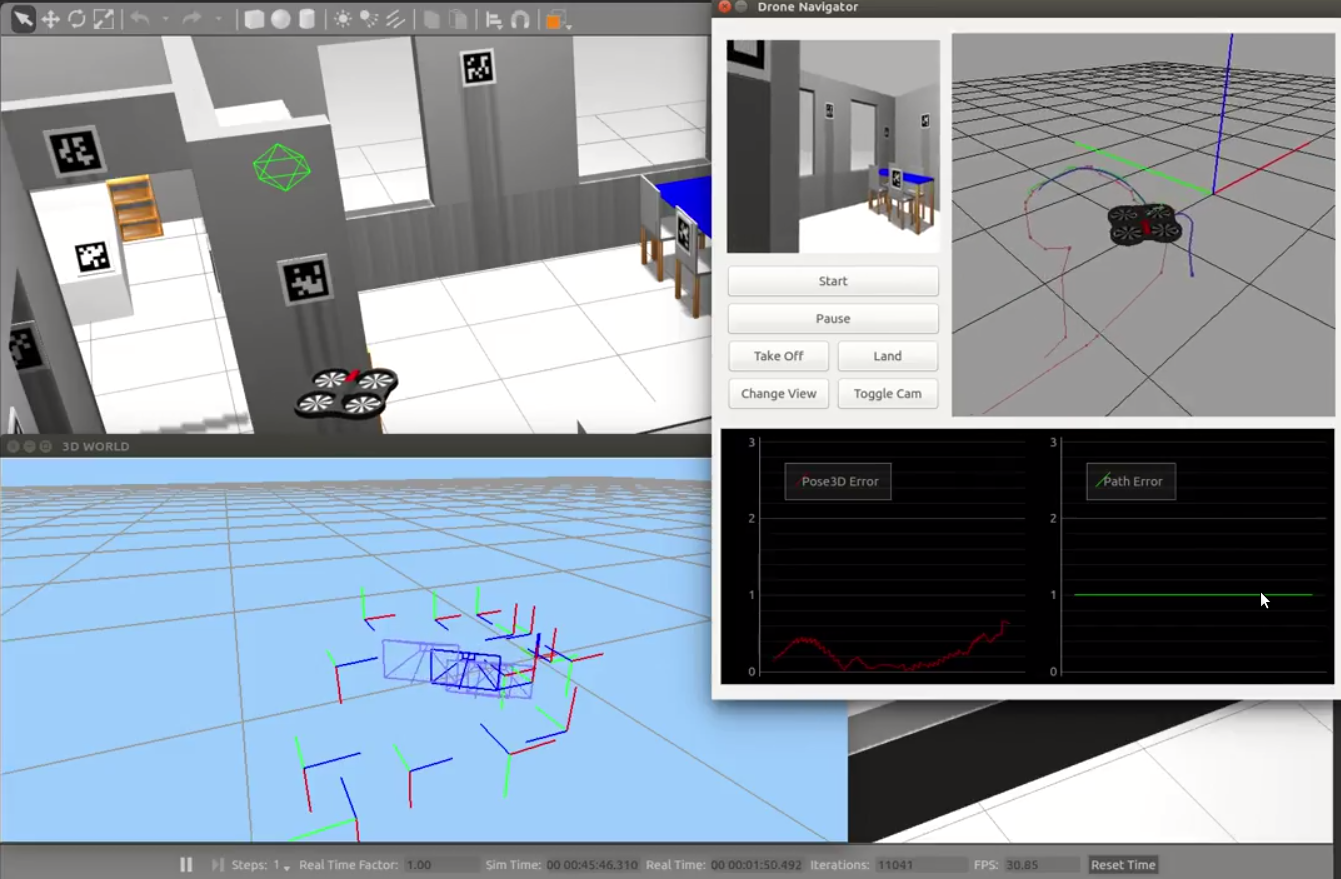
\includegraphics[width=12cm]{simnavigation.png}}
		\end{center}
                \label{fig:simnavigation}
		\caption{Position based control of a simulated drone}
	\end{figure}

% experimentos con drone real
	The first real scenario experiments showed an unstable system behavior, so several iterations had to be run in order to find the correct parameters. Starting with self-localization algorithm, noise matrixes had to be re-adjusted so they could reflect the new noise model. Several marker sizes were tested (17cm., 23cm.  and 33cm.), obtaining the best results with a 33cm. marker size. Also, quadcopter camera needed to be calibrated. The position control component also showed an erratic behaviour due to the natural drift of the vehicle and the magnitude of the velocity commands. Even though the drift caused by the slow movement of the vehicle could not be completeley countered, speed parameters were adjusted so its impact was minimal. Furthermore, the movement of the vehicle caused a blurry effect on cameras, being angular speed a critical factor for this incidence.
	
	\begin{figure}[h]
		\begin{center}
		{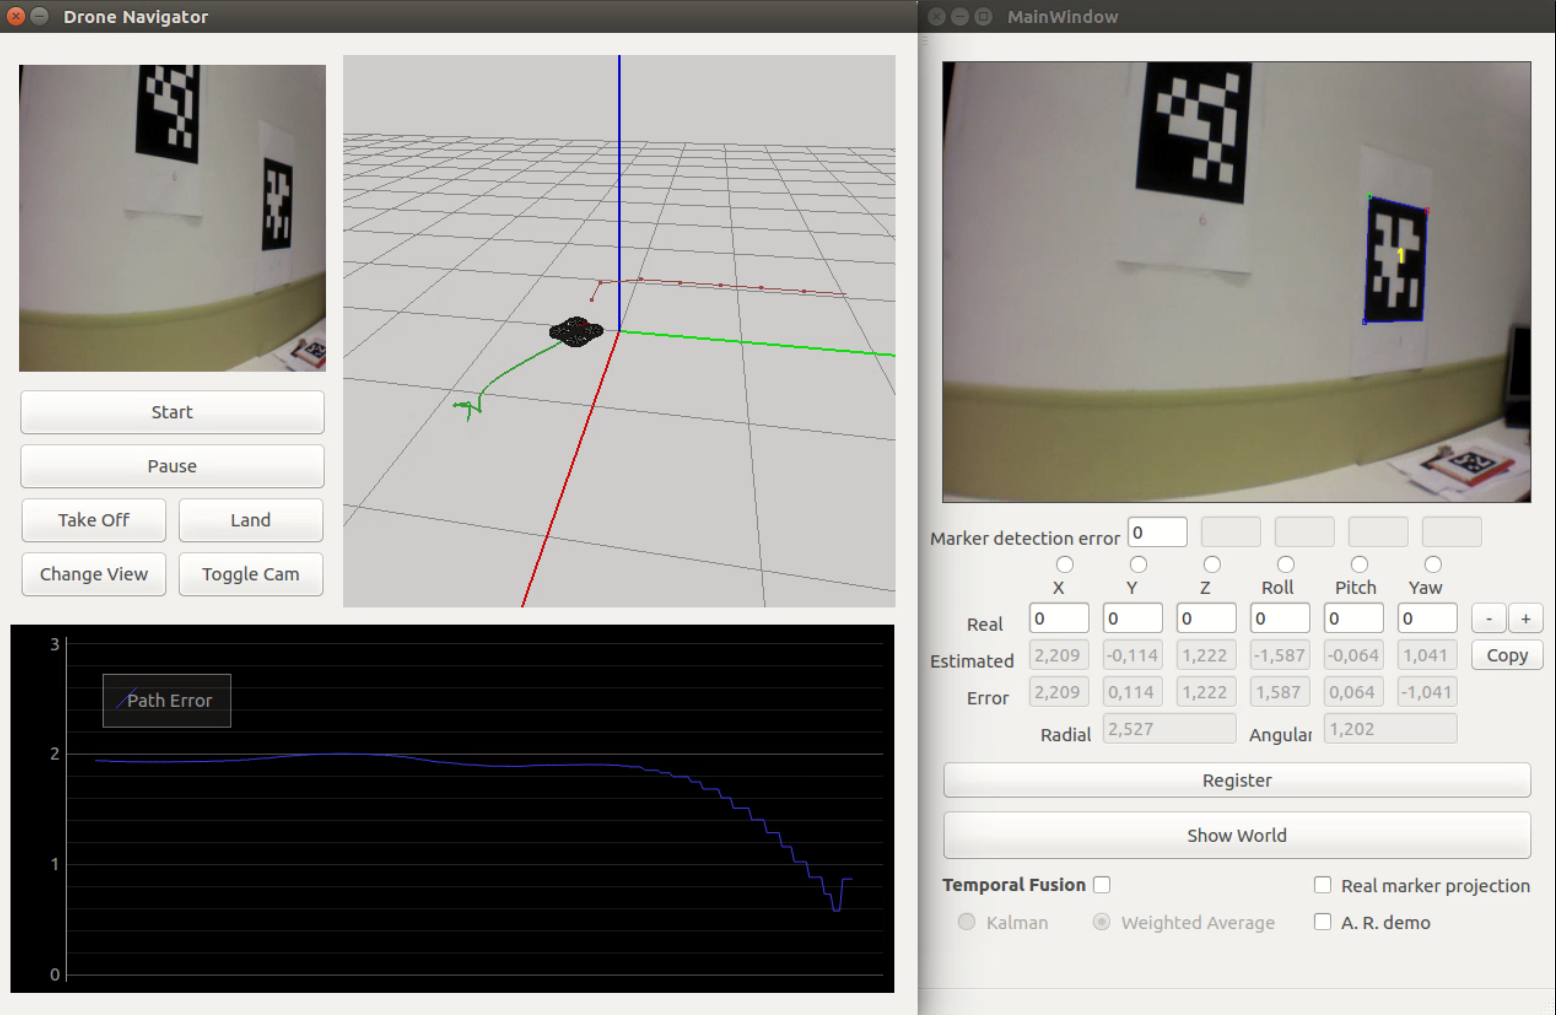
\includegraphics[width=12cm]{appcapture.png}}
		\end{center}
		\caption{Position based control of the real drone}
	\end{figure}


\section{Conclusions}

	We have designed and developed an autonomous quadricopter indoor flight system based on a fiducial auto-localization technique. In order to achieve that, we made use of a wide range of different technologies that had to be comprehended and sometimes adapted for our purposes. The system is validated on simulated environments as well as on real environments. Even though noisy data can affect the performance, it has been proven to be stable enough to fit the proposed goals.
	
	Experimental results show us that the system is limited in velocity due to the blurriness present in the images taken at high speed. Another limiting key factor to having a robust system is the size of the markers. Acknowledging those limitations, the final prototype is robust enough to satisfy the initial requirements of the project. Future working lines may involve the addition and combination of other visual auto-location techniques such as visual odometry. Furthermore, more exhaustive position control methods could be added in order to counter the quadricopter's drift.


        \section*{Acknowledgements}
%
% ---- Bibliography ----
%
\begin{thebibliography}{6}
\bibitem{wu2013}
Wu, A., Johnson, E.N., Kaess, M., Dellaert, F., Chowdhary, G.: Autonomous Flight in GPS-Denied Environments Using Monocular Vision and Inertial Sensors. J. Aerospace Inf. Sys.. 2013 Apr 1;10(4):172-86.

\bibitem{apvrille2013}
Apvrille, L., Dugelay, J.L., Ranft, B.: Indoor autonomous navigation of low-cost mavs using landmarks and 3d perception. Proc. Ocean and Coastal Observation, Sensors and Observing Systems. 2013 

\bibitem{forster2014}
Forster, C., Pizzoli, M., Scaramuzza, D.: SVO: Fast semi-direct monocular visual odometry, in Robotics and Automation (ICRA), 2014
IEEE International Conference on. IEEE, 2014, pp. 15–22.

\bibitem{engel2017}
J., Engel, Koltun, V., Cremers, D.,: Direct sparse odometry, IEEE Transactions on Pattern Analysis and Machine Intelligence, 2017

\bibitem{beul2015}
Beul, M., Krombach, N., Zhong, Y., Droeschel, D., Nieuwenhuisen, M., Behnke, S.: A High-performance MAV for Autonomous Navigation in Complex 3D Environments, International Conference on Unmanned Aircraft Systems (ICUAS) June 2015 \url{DOI: 10.1109/ICUAS.2015.7152417}

\bibitem{nikolic2014}
Nikolic, J., Leutenegger, S., Burri, M., Huerzeler, C., Rehder, J., Siegwart, R.: A UAV System for Inspection of Industrial Facilities, IEEE Aerospace Conference, 2013 \url{10.1109/AERO.2013.6496959}

\bibitem{lupashin2014}
Lupashin, S., Hehn, M., Mueller, M., Schoellig, A., Sherback, M., D’Andrea, R.: A platform for aerial robotics research and demonstration: The Flying Machine Arena, Mechatronics 24 (2014) 41–54

\bibitem{jimenez2014}
Jiménez, J., Zell, A.: Framework for Autonomous On-board Navigation with the AR.Drone, Journal of Intelligent \& Robotic Systems, January 2014, Volume 73, Issue 1–4, pp 401–412

\bibitem {dandrea2015}
Hehn, M., D'Andrea, R.: Real-Time Trajectory Generation for Quadrocopters, IEEE TRANSACTIONS ON ROBOTICS,  31(4), 2015

\bibitem {lopezceron2016}
López-Cerón, A., Cañas, J.M.: Accuracy analysis of marker-based 3D visual localization
 XXXVII Jornadas de Automática, Madrid, 2016 % \url{http://www.ncbi.nlm.nih.gov}

\bibitem{eolson}
Olson, E.: A robust and flexible visual fiducial system, IEEE International Conference on Robotics and Automation (ICRA), 3400-2407, 2011.

\end{thebibliography}

        
\end{document}

